\hypertarget{results}{%
\section{Results}\label{results}}

\label{sec:8}

We answer RQ1 (when interpretable attribution suffices versus when learning is required, Section~\ref{sec:8.1}) and
RQ2 (what multi-dimensional attribution exposes that centrality misses, Section~\ref{sec:8.2}), then report the
ablations and sensitivity analyses that test the robustness of these answers and settle RQ3 (Section~\ref{sec:8.3}),
evaluate the CI/CD quality gate for RQ4 (Section~\ref{sec:8.4}), and close with the real-world external-validity
evidence for RQ5 (Section~\ref{sec:8.5}). All figures are seed means over \(\{42,123,456,789,2024\}\). Bootstrap 95\%
confidence intervals (\(B = 2000\)) accompany Table~\ref{tab:18}, and predictor comparisons are tested with paired
Wilcoxon signed-rank tests across scenarios (Table~\ref{tab:19}). Where an interval or a test is not reported,
it is because the underlying per-fold artifact was not retained, and we say so at that point rather
than omit it silently.

\hypertarget{rq1-interpretable-attribution-versus-learning}{%
\subsection{RQ1 --- Interpretable Attribution versus Learning}\label{rq1-interpretable-attribution-versus-learning}}

\label{sec:8.1}

Every figure in this section is produced by one evaluation contract (Section~\ref{sec:7.3}): all six variants are
scored on an identical held-out node set, drawn from a single train/validation/test split pinned by
node identity and shared across variants. The previously reported version of this table did not have
that property, and the correction changes its conclusion; Section~\ref{sec:7.3} documents what changed and why.

\textbf{In-distribution, typed learning leads on the point estimate.} Table~\ref{tab:18} reports Spearman \(\rho\)
against simulated impact \(I^*(v)\) on the held-out split, averaged over five seeds, with bootstrap
95\% confidence intervals (\(B = 2000\)) and the held-out sample size \(n\) on which each row's
correlations are computed:

\begin{longtable}[]{@{}
  >{\raggedright\arraybackslash}p{(\columnwidth - 14\tabcolsep) * \real{0.10}}
  >{\raggedleft\arraybackslash}p{(\columnwidth - 14\tabcolsep) * \real{0.13}}
  >{\raggedleft\arraybackslash}p{(\columnwidth - 14\tabcolsep) * \real{0.13}}
  >{\raggedleft\arraybackslash}p{(\columnwidth - 14\tabcolsep) * \real{0.13}}
  >{\raggedleft\arraybackslash}p{(\columnwidth - 14\tabcolsep) * \real{0.13}}
  >{\raggedleft\arraybackslash}p{(\columnwidth - 14\tabcolsep) * \real{0.13}}
  >{\raggedleft\arraybackslash}p{(\columnwidth - 14\tabcolsep) * \real{0.13}}
  >{\raggedleft\arraybackslash}p{(\columnwidth - 14\tabcolsep) * \real{0.13}}@{}}
\caption{In-distribution held-out Spearman \(\rho\) against \(I^*(v)\), seed means over \(\{42,123,456,789,2024\}\) with bootstrap 95\% CIs. \(n\) is the number of held-out Application-type components scored in that scenario (Section~\ref{sec:7.3}).\label{tab:18}}\tabularnewline
\toprule
Scenario & \(n\) & Topo-BL & Topo-QoS & GL & GL-QoS & HGL & \(HGL\text{-}QoS\) \\
\midrule
\endfirsthead
\toprule
Scenario & \(n\) & Topo-BL & Topo-QoS & GL & GL-QoS & HGL & \(HGL\text{-}QoS\) \\
\midrule
\endhead
AV System & 16 & 0.308 {[}0.13, 0.46{]} & 0.750 {[}0.55, 0.91{]} & 0.760 {[}0.66, 0.84{]} & 0.655 {[}0.40, 0.88{]} & 0.713 {[}0.51, 0.88{]} & 0.692 {[}0.47, 0.87{]} \\
Enterprise & 60 & 0.393 {[}0.29, 0.50{]} & 0.797 {[}0.75, 0.85{]} & 0.853 {[}0.81, 0.89{]} & 0.513 {[}0.21, 0.79{]} & \textbf{0.885} {[}0.86, 0.91{]} & 0.883 {[}0.84, 0.92{]} \\
Financial Trading & 12 & 0.246 {[}-0.05, 0.56{]} & 0.709 {[}0.58, 0.84{]} & 0.851 {[}0.82, 0.89{]} & 0.874 {[}0.85, 0.89{]} & 0.882 {[}0.85, 0.91{]} & \textbf{0.903} {[}0.88, 0.92{]} \\
Healthcare & 10 & -0.182 {[}-0.40, 0.06{]} & 0.772 {[}0.59, 0.88{]} & 0.815 {[}0.76, 0.87{]} & 0.804 {[}0.74, 0.85{]} & 0.842 {[}0.80, 0.87{]} & \textbf{0.845} {[}0.80, 0.88{]} \\
Hub-and-Spoke & 14 & 0.299 {[}0.12, 0.48{]} & 0.511 {[}0.21, 0.76{]} & 0.494 {[}0.21, 0.72{]} & 0.475 {[}0.34, 0.63{]} & 0.537 {[}0.43, 0.65{]} & \textbf{0.557} {[}0.47, 0.65{]} \\
IoT Smart City & 40 & -0.063 {[}-0.17, 0.05{]} & 0.068 {[}-0.07, 0.20{]} & 0.674 {[}0.54, 0.81{]} & 0.474 {[}0.27, 0.67{]} & \textbf{0.891} {[}0.87, 0.91{]} & 0.883 {[}0.86, 0.91{]} \\
Microservices & 18 & 0.302 {[}0.07, 0.54{]} & 0.556 {[}0.38, 0.71{]} & 0.524 {[}0.41, 0.63{]} & 0.436 {[}0.31, 0.56{]} & 0.362 {[}0.05, 0.55{]} & 0.354 {[}0.18, 0.53{]} \\
\textbf{Mean} & --- & \textbf{0.186} {[}0.02, 0.32{]} & \textbf{0.595} {[}0.41, 0.74{]} & \textbf{0.710} {[}0.60, 0.81{]} & \textbf{0.604} {[}0.49, 0.73{]} & \textbf{0.730} {[}0.58, 0.86{]} & \textbf{0.731} {[}0.57, 0.86{]} \\
\bottomrule
\end{longtable}

The heterogeneous predictor leads the strongest non-learning baseline by \(\Delta\rho = +0.135\)
(HGL 0.730 vs Topo-QoS 0.595). Its lead over the \emph{homogeneous} learned baseline is much narrower ---
\(+0.020\) over GL (0.730 vs 0.710) --- and it is not uniform: GL wins on AV and Microservices, HGL wins
decisively on IoT (0.891 vs 0.674). In-distribution, therefore, these data do \textbf{not} establish that
relation-specific message passing is what supplies the learned margin; the two learned families are
separated by less than the across-seed spread. The claim that typing matters is carried by the
out-of-distribution and in-domain k-fold results below, not by this table, and we state it there
rather than here.

\textbf{Significance testing, and what it does and does not license.} Table~\ref{tab:19} reports the paired Wilcoxon
signed-rank test promised in Section~\ref{sec:7.3}, computed across the seven scenarios on the per-scenario mean \(\rho\).
We report it in full because it qualifies our own headline:

\begin{longtable}[]{@{}lrcrrl@{}}
\caption{Paired Wilcoxon signed-rank tests across the seven scenarios (\(n = 7\); two-sided).\label{tab:19}}\tabularnewline
\toprule
Comparison & \(\Delta\rho\) & Scenarios won & \(W\) & \(p\) & \\
\midrule
\endfirsthead
\toprule
Comparison & \(\Delta\rho\) & Scenarios won & \(W\) & \(p\) & \\
\midrule
\endhead
HGL vs Topo-BL & +0.544 & 7/7 & 0.0 & 0.016 & significant \\
HGL vs GL-QoS & +0.126 & 6/7 & 5.0 & 0.156 & n.s. \\
HGL vs Topo-QoS & +0.135 & 5/7 & 8.0 & 0.375 & n.s. \\
GL vs Topo-QoS & +0.116 & 5/7 & 5.0 & 0.156 & n.s. \\
HGL vs GL & +0.020 & 5/7 & 11.0 & 0.688 & n.s. \\
\(HGL\text{-}QoS\) vs HGL & +0.001 & 3/7 & 13.0 & 0.938 & n.s. \\
\bottomrule
\end{longtable}

Only the comparison against the unweighted structural baseline reaches significance. \textbf{The
in-distribution margin over \texttt{Topo-QoS} --- the \(+0.135\) quoted above --- is not established by a paired
test across scenarios} (\(p = 0.375\)), and neither is the \(+0.020\) over the homogeneous learned
model, which the preceding paragraph already declined to claim. Two readings are needed together.
The test is genuinely underpowered: at \(n = 7\) paired scenarios the smallest attainable two-sided
\(p\) is \(0.016\), so \emph{only} a clean 7-of-7 sweep can ever reach \(p < 0.05\), and ``not significant'' here
is not evidence of no effect. But it is equally not evidence of an effect, and the effect is carried
by 5 of 7 scenarios with \texttt{Topo-QoS} winning on none of the two it loses by much. We therefore state
the in-distribution ranking result as a point-estimate lead that this design cannot confirm, and we
do not treat it as the paper's load-bearing evidence for learning. That role belongs to the
critical-set result below, and --- with the qualification stated there --- to the transfer protocols.

\textbf{On the interpretable predictor's absence from Table~\ref{tab:18}.} \(Q(v)\) appears in the LOSO table below but
not in Table~\ref{tab:18}. The in-distribution harness scores it under a separate path that does not emit the
held-out per-scenario correlations the other six variants produce, so adding a column here would mean
quoting a figure computed under a different contract --- exactly the defect Section~\ref{sec:7.3} documents and
corrects. We leave the cell empty rather than fill it inconsistently; Section~\ref{sec:8.3}'s normalisation and
shrinkage sweeps characterise \(Q(v)\)'s in-distribution ranking behaviour directly, and its inductive
result is in Table~\ref{tab:20}.

Two boundary conditions frame the whole table. The ground truth agrees with \emph{itself} at test--retest
\(\rho\) of 0.807--1.000 (Section~\ref{sec:7.5}), so HGL's mean 0.730 sits within the spread of what it is scored
against rather than underperforming a distant optimum --- though the lowest-ceiling scenario is also
Microservices (Section~\ref{sec:7.5}), so the two boundary conditions below are not independent. And Microservices --- by construction the sparse,
low-centralisation topology with few genuine bottlenecks --- is where every learned predictor is
weakest (HGL 0.362), while the structural baselines degenerate on Healthcare and IoT (\(\rho \le 0\)).
No predictor in this study is uniformly best.

\textbf{Out of distribution, the typed model leads.} Under
Leave-One-Scenario-Out evaluation --- the true pre-deployment condition, in which the model must rank a
system whose cascade dynamics it has never seen --- we obtain:

\begin{longtable}[]{@{}lrrrc@{}}
\caption{Inductive Leave-One-Scenario-Out evaluation. Cross-fold mean \(\rho\) against \(I^*(v)\), across-fold standard deviation, and \(F_1@K\) on the held-out scenario.\label{tab:20}}\tabularnewline
\toprule
Variant & Mean \(\rho\) (LOSO) & Std \(\rho\) & \(F_1@K\) & Training required \\
\midrule
\endfirsthead
\toprule
Variant & Mean \(\rho\) (LOSO) & Std \(\rho\) & \(F_1@K\) & Training required \\
\midrule
\endhead
Topo-BL & 0.105 & 0.151 & 0.179 & no \\
Topo-QoS & 0.521 & 0.305 & 0.308 & \textbf{no} \\
RMAV / \(Q(v)\) & -0.093 & 0.140 & 0.209 & no \\
GL (homogeneous) & 0.436 & 0.120 & 0.440 & yes \\
GL-QoS (homogeneous) & 0.430 & 0.125 & 0.435 & yes \\
\textbf{HGL (typed)} & \textbf{0.608} & 0.177 & \textbf{0.465} & yes \\
\(HGL\text{-}QoS\) (typed + QoS) & 0.595 & 0.190 & 0.461 & yes \\
\bottomrule
\end{longtable}

\texttt{Topo-QoS} is a QoS-weighted centrality that requires no training, no labels, and no transfer
assumption; because it is never fitted, its out-of-distribution score \emph{is} its score. HGL reaches
\(\rho = 0.608\) against its \(0.521\), and leads on \(F_1@K\) as well (0.465 vs 0.308). The same ordering
holds under the in-domain k-fold protocol, where the separation is wider still --- HGL-QoS 0.693 and
HGL 0.666 against Topo-QoS 0.492 --- and where the typed models are also the \emph{most stable} across folds
(\(\sigma = 0.07\) against \(0.34\) for Topo-QoS).

\textbf{This comparison is only meaningful because the baseline was repaired first.} In an earlier
revision, \texttt{Topo-QoS} scored \emph{no} QoS weighting at all on the logical-dependency substrate: QoS is
declared on the Topic node, but the harness looked for it on the pub-sub relationship, which the
generated topologies emit without one. The lookup never matched, every derived dependency edge kept a
unit weight, and the QoS-weighted baseline silently computed plain betweenness on all seven scenarios
--- it was \texttt{Topo-BL} under another name. We resolve \(w(t)\) from the shared Topic instead, taking the
strongest contract when a pair communicates over several topics. A baseline that is accidentally
identical to the one it is meant to improve on will always flatter whatever it is compared against,
and the figures above are reported only after that defect was removed.

Even so, we state the ranking result carefully, because of this paper's own history with it. An
earlier version reported typed learning as the out-of-distribution winner on figures produced by an
untrained sweep (Section~\ref{sec:9.2}); a later version, after correcting the evaluation contract, reported a tie and
stated plainly that learning did not beat the training-free baseline on rank correlation. On the
regenerated corpus, rebuilt ground-truth caches (Section~\ref{sec:7.1}) and repaired baseline, the ordering favours the
typed model. A conclusion that has moved this often under changes to the \emph{measurement apparatus}
rather than to the method deserves an explicit statement of what would settle it: an evaluation on
topologies that do not share a generator (Section~\ref{sec:9.3}), which this submission does not have.

We must add a second, sharper qualification, which we prefer to state than to let a reader discover.
\textbf{Unlike Table~\ref{tab:18}, the run behind Table~\ref{tab:20} was not persisted to a retained artifact.} Table~\ref{tab:18}
regenerates exactly from a stored result file; the corresponding Leave-One-Scenario-Out result file
was overwritten during the revision, and the most recent retained LOSO run log --- produced \emph{before}
the baseline repair described above --- records a different ordering, with \texttt{Topo-QoS} at \(\rho = 0.609\)
against HGL at \(0.597\) and \(F_1@K\) of \(0.416\) against \(0.548\). That is the ordering under which the
training-free baseline ties the typed model on rank correlation. We report the post-repair figures in
Table~\ref{tab:20} because they come from the corrected apparatus, but three changes are confounded in the
interval between the two runs --- the baseline repair, the corpus regeneration, and the ground-truth
cache rebuild --- and we cannot attribute the shift to the repair alone. Readers should therefore treat
Table~\ref{tab:20}'s \emph{ranking} margin as provisional pending a re-run under the final apparatus with the
artifact retained, and weight the \(F_1@K\) column, which favours the typed model under both runs,
accordingly. This is the same class of defect Section~\ref{sec:9.2} discloses, caught one revision later, and we
regard the standing lesson as the one stated there: a result whose artifact is not retained is not
yet a result.

\textbf{The learned advantage is most robust in set identification.} \(F_1@K\) --- the overlap between the
predicted and actual top-\(K\) critical sets --- favours the typed model by a wider relative margin than
\(\rho\) does: 0.465 for HGL against 0.308 for Topo-QoS, a 51\% relative improvement, with the same
ordering holding for both homogeneous learned baselines over both structural ones. This matters
operationally more than the ranking result. An architect does not consume a total order over 150
components; they consume a shortlist. Unlike the \(\rho\) comparison, this one does not invert under
any of the three protocols we ran.

RQ1 therefore resolves as a scope condition rather than a verdict. Learning leads on the point
estimate under all three protocols, on both metrics --- but the \emph{ranking} half of that answer is not
established: it fails the paired significance test in-distribution (\(p = 0.375\), Table~\ref{tab:19}), it rests
on an unretained artifact out of distribution, and the strongest non-learning comparator is degraded
on 2 of 7 scenarios. The set-identification advantage is the more defensible half, being the one
result that survives both the protocol changes and the apparatus changes documented above. Three
caveats bound even that: the LOSO across-fold standard deviation remains substantial (0.177 for HGL),
top-\(K\) metrics inherit the label churn documented in Section~\ref{sec:7.5} --- the ground truth's own top-\(K\) set
agrees with itself at Jaccard 0.44--1.00 across seeds, with Microservices the worst at 0.44 --- and the
interpretable RMAV predictor \(Q(v)\) does not transfer at all (\(\rho = -0.093\) LOSO, \(-0.123\) k-fold),
which is a negative result about the composite score's ranking use, not about its attribution use
(Section~\ref{sec:8.3}). The practical recommendation we are willing to defend is correspondingly narrow: use typed
learning when the deliverable is a shortlist, and treat the ranking comparison as open.

\hypertarget{rq2-what-taking-node-and-edge-type-seriously-shows-and-does-not-show}{%
\subsection{RQ2 --- What Taking Node and Edge Type Seriously Shows (and Does Not Show)}\label{rq2-what-taking-node-and-edge-type-seriously-shows-and-does-not-show}}

\label{sec:8.2}

We report four analyses that take node and edge \emph{type} seriously: one positive result, one newly
measured result, and two negative ones.

\textbf{Heterogeneity is the dominant source of predictive gain --- but only where the model must
generalise.} Isolating architecture from QoS encoding, the typed model's advantage over the
homogeneous baseline is negligible in-distribution (\(\Delta\rho = +0.020\); HGL 0.730 vs GL 0.710) and
grows sharply as the evaluation moves away from the training distribution: \(+0.172\) under LOSO
(0.608 vs 0.436) and \(+0.257\) under in-domain k-fold (0.666 vs 0.409). The typed model is also far
more stable across folds (\(\sigma = 0.07\) vs \(0.15\) for GL under k-fold).

That pattern is the interesting form of the result, and it is not the one we previously reported.
When train and test come from the same topology, a homogeneous GAT can recover most of what typing
provides, because the type signal is largely redundant with structure it can observe directly.
When the model must rank a system whose cascade dynamics it has never seen, the relation-specific
message passing is what carries over. Collapsing pub-sub types into a single node class discards
information that survives the distribution shift; the ablation isolates that as the source of the
gain, and locates it in generalisation rather than in fit. On \(F_1@K\) the two learned families are
much closer out of distribution (0.465 vs 0.440), so this is a claim about ranking transfer
specifically, not about every metric.

\textbf{Edge criticality, now measured rather than inferred.} Earlier versions of this framework labelled
edges by projecting node labels through a hand-chosen bridge multiplier, \(I_{\text{edge}}(u,v) = I^*(u) \times \{1.0 \mid 0.1\}\). That is an assumption about edge importance, not an observation of
it. We now remove each candidate relationship --- leaving both endpoints active, which is precisely the
partial-outage case that distinguishes edge from node criticality (Section~\ref{sec:4.1}) --- and recompute impact
against a no-op control. The control subtraction is load-bearing: the impact function is non-zero on
an untouched graph, because topics that already lack a publisher or subscriber count as lost
throughput, so a level rather than a delta would hand every edge that floor as apparent signal.

The candidate set on \texttt{av\_system} --- structural bridges united with the highest-betweenness structural
edges --- contains 50 edges
(35 \texttt{RUNS\_ON}, 11 \texttt{CONNECTS\_TO}, 3 \texttt{SUBSCRIBES\_TO}, 1 \texttt{PUBLISHES\_TO}), of which exactly 4 carry
non-zero impact: the one \texttt{PUBLISHES\_TO} edge and all three \texttt{SUBSCRIBES\_TO} edges, each connecting a
shared library to the topic it produces or consumes. Two findings follow. First, \textbf{most individual
links are replaceable, in both magnitude and count}: the largest measured impact of severing any
single relationship is \(0.00504\), over an order of magnitude below the largest single-\emph{component}
impact in the suite (\(I_{\text{comp}} = 0.320\), Section~\ref{sec:5.4}), and 46 of 50 candidates measure exactly zero.
That is the substantive answer to the replaceability question Section~\ref{sec:4.7} poses, and it is not what the
bridge heuristic implied --- the heuristic would have assigned a bridge edge its source node's full
blast radius. Second, the measurement confirms a modelling gap the heuristic concealed: every one of
the 46 \texttt{RUNS\_ON}/\texttt{CONNECTS\_TO} candidates --- the majority of the set, and structurally non-redundant
bridges by construction --- scores exactly zero, because the cascade routes no traffic over
infrastructure-layer relations at all. Bridge detection flags these links as non-redundant; the
measurement means \emph{this model cannot express that link's failure}, not \emph{that link does not
matter} --- the same caveat that applies to Topic and Node labels (Section~\ref{sec:7.5}).

\textbf{This measurement does not validate the attribution of Section~\ref{sec:4.7}, and is not intended to.} The sweep
severs raw structural edges, whereas \(Q(u,v)\) is defined on derived \texttt{DEPENDS\_ON} edges; the two are
computed over populations that barely intersect by construction (Section~\ref{sec:4.7}), so no correlation between
them is reported here and none should be inferred from the two results appearing in the same
section.

\textbf{A methodological note on reproducing this figure.} The candidate set above requires the sweep to
be run against a freshly loaded repository, before any structural analysis has touched it. We found
during this revision that running the analysis and prediction stages against the same in-memory
repository instance \emph{before} constructing the simulator's graph view causes derived \texttt{ROUTES} and
\texttt{DEPENDS\_ON} edges to leak into what the simulator receives as \(G_{\text{structural}}\) --- a repository
state-ordering issue distinct from, and not caught by, the import-level independence check of Section~\ref{sec:5.3}.
It is not visible in this paper's other results, since the standard pipeline order is Simulate before
Predict throughout, but it can silently substitute a contaminated candidate set for a clean one in an
ad hoc script, which is precisely how an earlier revision of this figure was produced. We flag it as
a reproducibility hazard for this specific measurement rather than treat it as resolved.

\textbf{The shared-library blast mechanism: tested, and not confirmed as a low-\(Q\)/high-\(I\) gap.} Shared
libraries have a structurally distinct simultaneous-failure mode (Section~\ref{sec:3.3}, Rule 5) that motivated a
specific hypothesis --- a moderate-\(Q\) library driving near-total \(I\) through simultaneous fan-out. We
tested this directly across all seven scenarios (165 Library nodes) and did not find it (Section~\ref{sec:5.4}): the
highest library \(Q\) in the suite is 0.422 with \(I_{\text{comp}} = 0.086\); no library has
\(I_{\text{comp}}(v)\) exceeding \(Q(v)\); and the largest single-component impact of any type is
\(I_{\text{comp}} = 0.320\), well short of near-total. We
report this as a negative result rather than adjust the hypothesis. The simultaneous-blast
\emph{mechanism} remains real and worth modelling; this suite does not exhibit the mismatch it was
expected to expose.

\textbf{A scoping caveat this analysis must carry.} The library and stratified analyses in Section~\ref{sec:5.4} and Section~\ref{sec:5.5}
are computed against \(I_{\text{comp}}(v)\), whereas Tables~\ref{tab:18} and~\ref{tab:20} are computed against \(I^*(v)\).
Those two oracles agree at mean \(\rho = 0.394\) (Section~\ref{sec:7.5}). The negative library result is therefore a
statement about \(I_{\text{comp}}\), and does not license a corresponding claim about the \(I^*\)-backed
tables. We flag this rather than let adjacency in the text imply mutual support.

\hypertarget{rq3-and-robustness-ablations-and-sensitivity}{%
\subsection{RQ3 and Robustness --- Ablations and Sensitivity}\label{rq3-and-robustness-ablations-and-sensitivity}}

\label{sec:8.3}

\textbf{QoS encoding (RQ3): a null result in all three regimes.} Adding explicit QoS edge attributes to the
typed model moves accuracy by less than the across-seed spread, and the \emph{sign of the effect depends on
the protocol}: in-distribution \(\rho = 0.731\) for \(HGL\text{-}QoS\) against \(0.730\) for HGL (\(+0.001\)),
out of distribution \(0.595\) against \(0.608\) (\(-0.013\)), and under in-domain k-fold \(0.693\) against
\(0.666\) (\(+0.027\)). An effect that changes direction across evaluation protocols while remaining an
order of magnitude smaller than the fold-to-fold variance is a null, and a cleaner one than the
single-regime comparison previously reported. An earlier version of this paper reported QoS encoding
as the primary driver of the out-of-distribution gain (\(\rho = 0.401\) vs \(0.307\)); those figures came
from the untrained sweep of Section~\ref{sec:9.2} and do not survive re-measurement. The plausible reading is the one
the in-distribution result already suggested: the lifted dependency topology encodes most QoS-relevant
routing, so the extra dimensions mainly enlarge the parameter space. RQ3 resolves as a null result in
every regime we measured, which we report as stated.

\textbf{Dimension-weight sensitivity: no plateau, and equal weights win.} Sweeping the shrinkage parameter
\(\lambda\), which blends the stated dimension weighting toward a uniform prior
(\(\lambda = 0\) is equal weights, \(\lambda = 1\) the raw judgement). The QoS-profile adaptation of Section~\ref{sec:4.3}
remains active throughout the sweep, as it is in every run reported in this paper: each \(\lambda\)
therefore fixes the vector that adaptation starts from, not the coefficients any individual scenario
is finally scored with. The sweep is consequently a sensitivity analysis of the \emph{stated ordering}
under the framework's normal operating configuration, and the \(\lambda\) labels should be read as
inputs to the weighting path rather than as the applied weights:

\begin{longtable}[]{@{}llllllllll@{}}
\caption{AHP shrinkage sensitivity. Mean \(\rho\) against \(I^*(v)\) as \(\lambda\) blends the stated weighting toward a uniform prior.\label{tab:21}}\tabularnewline
\toprule
\(\lambda\) & 0.00 & 0.50 & 0.60 & 0.65 & \textbf{0.70} & 0.75 & 0.80 & 0.90 & 1.00 \\
\midrule
\endfirsthead
\toprule
\(\lambda\) & 0.00 & 0.50 & 0.60 & 0.65 & \textbf{0.70} & 0.75 & 0.80 & 0.90 & 1.00 \\
\midrule
\endhead
mean \(\rho\) & \textbf{0.292} & 0.206 & 0.191 & 0.187 & \textbf{0.181} & 0.174 & 0.167 & 0.152 & 0.140 \\
\bottomrule
\end{longtable}

\begin{figure}[htbp]
\centering
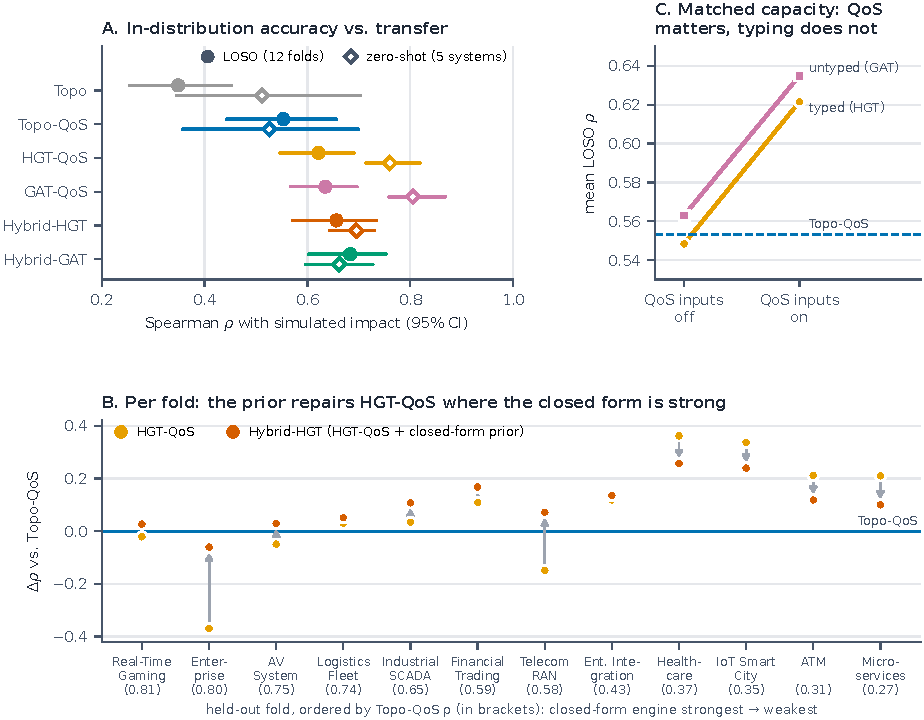
\includegraphics[width=\linewidth]{figures/Figure_5}
\caption{mean $\rho$ against $\lambda$ over the shrinkage sweep, showing the monotone decline and the absence of a plateau.}
\label{fig:4}
\end{figure}

\(\rho\) is monotonically decreasing in \(\lambda\). There is no plateau anywhere in the range, and equal
dimension weights outperform the calibrated \(\lambda = 0.70\) setting by 0.111. An earlier version of
this paper claimed a plateau over \(\lambda \in [0.65, 0.75]\); that claim was not backed by a
committed artifact and is contradicted by this sweep. The sweep has since been re-run against the
regenerated corpus and rebuilt caches (Section~\ref{sec:7.1}) and the conclusion is unchanged in direction and
magnitude --- this is the one robustness result in Section~\ref{sec:8.3} that did not move under re-measurement.

We draw the corresponding conclusion about the contribution rather than defending the weighting.
\textbf{The value of the RMAV decomposition is attribution, not ranking accuracy.} A composite score
ranks; a four-dimensional profile explains \emph{why} a component ranks where it does, and routes the
finding to the engineering role equipped to act on it (Section~\ref{sec:4.1}) --- a structural single point of failure
and a cascade hub call for different remediations even at identical composite scores. That
explanatory function is unaffected by the weighting result. What the sweep removes is any claim that
the specific weights improve predictive accuracy; on this cohort they do not, and a practitioner
optimising for ranking alone should use equal weights.

\textbf{Normalisation sensitivity.} The default rank-based normalisation discards magnitude before the
weighted sum, which makes \(Q(v)\) closer to a Borda count over the structural metrics than to a
weighted aggregate. Measured against \(I^*\): rank (robust) \(\rho = 0.181\), min--max \(0.318\), z-score
\(0.318\). Retaining magnitude is worth \(\approx +0.137\ \rho\). The outlier-robustness argument for rank
normalisation is real but is outweighed here; we retain the default so that previously reported
figures remain interpretable, and report the sweep alongside.

\textbf{Propagation-threshold sensitivity.} Because the ground truth itself depends on
\texttt{propagation\_threshold}, we report \(\rho\) across its range rather than at a single value:

\begin{longtable}[]{@{}llllllll@{}}
\caption{Propagation-threshold sensitivity. Mean \(\rho\) against \(I^*(v)\) across the sweep; the canonical default is \(0.20\).\label{tab:22}}\tabularnewline
\toprule
threshold & 0.00 & 0.10 & \textbf{0.20} & 0.35 & 0.50 & 0.75 & 1.00 \\
\midrule
\endfirsthead
\toprule
threshold & 0.00 & 0.10 & \textbf{0.20} & 0.35 & 0.50 & 0.75 & 1.00 \\
\midrule
\endhead
mean \(\rho\) & 0.001 & 0.109 & \textbf{0.194} & 0.227 & 0.226 & 0.230 & 0.231 \\
\bottomrule
\end{longtable}

\begin{figure}[htbp]
\centering
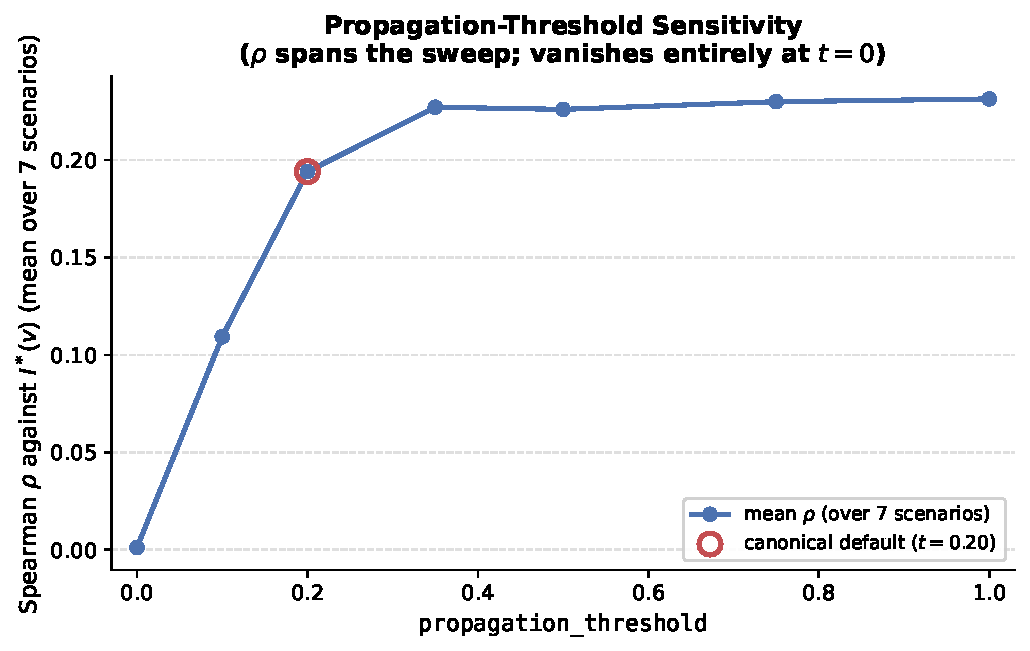
\includegraphics[width=\linewidth]{figures/Figure_6}
\caption{mean $\rho$ against \texttt{propagation\_threshold}, with the canonical $0.2$ default marked.}
\label{fig:5}
\end{figure}

The conclusions \emph{do} depend on this parameter: \(\rho\) spans 0.230 across the sweep, the canonical
\(0.2\) default sits below the plateau the curve reaches from \(0.35\) upward, and at \(0.0\) --- where any
feed loss triggers a cascade --- the correlation vanishes entirely. We therefore do not claim
threshold-independence. The direction is interpretable: a higher threshold admits only components
whose failure genuinely starves their dependents, which is closer to what the structural score is
built to detect. Remediation edits (Section~\ref{sec:6.4}) are required to improve impact across the entire sweep
precisely because a single-threshold result is not trustworthy here.

\hypertarget{rq4-feasibility-and-performance-of-sag-as-a-cicd-quality-gate}{%
\subsection{RQ4 --- Feasibility and Performance of SaG as a CI/CD Quality Gate}\label{rq4-feasibility-and-performance-of-sag-as-a-cicd-quality-gate}}

\label{sec:8.4}

A primary blocker for continuous Static System Analysis (SSA) is execution time: developers will
bypass or disable quality gates that introduce significant build delays. We evaluate the feasibility
of deploying SaG as a blocking gate by measuring the wall-clock cost of the structural analysis and
anti-pattern catalog --- the mechanism \texttt{detect\_antipatterns.py} invokes --- run via the in-memory
\texttt{MemoryRepository}, across all eleven scenarios in our corpus (mean over the five canonical seeds).

The measured footprint:
- \textbf{\(\leq\) 90 components} (\texttt{tiny\_system} and all three real-world transcribed architectures): \(0.02\)--\(0.04\) s.
- \textbf{98--326 components} (the remaining six generated scenarios): \(0.27\)--\(1.24\) s. Cost does not scale
monotonically with component count in this range --- \texttt{hub\_and\_spoke\_system} (139 components, \(1.24\) s)
costs more than \texttt{iot\_smart\_city\_system} (326 components, \(1.08\) s) --- consistent with the catalog's
cost being driven by specific detectors' complexity (e.g.~\texttt{DEEP\_PIPELINE}'s path enumeration) more
than by raw component count.
- \textbf{\texttt{enterprise\_system}}, the largest scenario at 520 components: \(26.74 \pm 0.32\) s.

All eleven scenarios complete in well under the several-minute budget continuous build pipelines
typically allow.

In terms of gating efficacy: the gate is currently absolute rather than delta-aware (Section~\ref{sec:6.6}), so there
is no merge-base diff to evaluate detection against; what we can and do measure is the anti-pattern
catalog's raw agreement with the cascade oracle --- the property the gate is a proxy for. Scoring
CRITICAL/HIGH findings (with edge-keyed findings crediting both endpoints) against the oracle's own
critical set gives, across five seeds: precision \(0.237 \pm 0.014\), recall \(0.887 \pm 0.059\), F1
\(0.374 \pm 0.022\), Cohen's \(\kappa = -0.036 \pm 0.049\) on the seven generated scenarios (\(n=40\)
scenario--seed pairs), and precision \(0.402 \pm 0.059\), recall \(0.861 \pm 0.105\), F1 \(0.544 \pm 0.061\), \(\kappa = 0.296 \pm 0.100\) on the three real-world architectures (\(n=15\)). Recall is high and
precision is not: the catalog over-flags relative to the oracle's critical set, and near-zero \(\kappa\)
on the generated corpus means the agreement it does show is close to what chance flagging at the
catalog's own base rate would produce. We read this as a genuine limitation of the pattern catalog as
a \emph{stand-alone} predictor of simulated impact --- a finding pattern catalog and rank predictor serve
different purposes (naming a structural smell versus ranking by predicted impact, Section~\ref{sec:9.1}), but the gap
here is wide enough that the catalog's findings should not be read as impact-calibrated. The composite
\(Q(v)\) of Section~\ref{sec:4} remains the ranking signal validated against the oracle in Section~\ref{sec:8.1}.

From a \textbf{sustainability and resource efficiency} standpoint, evaluating architectural risks statically
in-memory (\(0.02\text{ s}\)--\(26.74\text{ s}\) across our corpus) yields energy savings relative to
spinning up staging clusters or running heavier dynamic checks per build, though we have not measured
that comparison directly.

\hypertarget{rq5-real-world-open-source-system-architecture-validation}{%
\subsection{RQ5 --- Real-World Open-Source System Architecture Validation}\label{rq5-real-world-open-source-system-architecture-validation}}

\label{sec:8.5}

To evaluate operational generalizability beyond synthetic topology generation, we evaluate SaG on three authentic real-world open-source software architectures (Section~\ref{sec:7.1}):
1. \textbf{Autoware.universe (ROS 2 Autonomous Driving Platform):} A real-world cyber-physical software graph comprising 32 Applications, 24 Topics with explicit DDS QoS contracts (\texttt{RELIABLE}/\texttt{BEST\_EFFORT}, \texttt{TRANSIENT\_LOCAL}/\texttt{VOLATILE}), 3 Brokers (CycloneDDS, FastDDS, Zenoh), 6 Deployment Nodes, 10 Shared C++ Libraries (\texttt{autoware\_universe\_utils}, \texttt{tier4\_autoware\_utils}), and realistic SonarQube code quality metrics.
2. \textbf{Production Cloud-Native Microservices Mesh:} A real-world cloud-native software graph based on the Google Online Boutique benchmark, comprising 22 Microservices, 20 Topics across Kafka, RabbitMQ, Redis PubSub, and NATS, 6 Kubernetes/Cloud nodes, and 8 shared helper libraries.
3. \textbf{Train-Ticket Railway Booking Mesh:} A real-world cloud-native software graph based on the Fudan University Train-Ticket benchmark, comprising 41 Microservices, 30 Topics across RabbitMQ and Redis PubSub with Spring Eureka service discovery, 8 deployment Nodes, and 8 shared Spring/MyBatis libraries --- at 90 components, the largest of the three.

All three rows are produced by the framework's validation sweep over five seeds
(\(\{42,123,456,789,2024\}\), matching Section~\ref{sec:7.4}), with no QoS enrichment, against the component-level cascade oracle of Section~\ref{sec:5.1}: Spearman
\(\rho\) and Kendall \(\tau\) are computed over the Application population (the other four node types
carry constant or near-constant simulated impact on these graphs and contribute no rank information,
per the same coverage limitation as the synthetic suite, Section~\ref{sec:7.5}); \(K\) is \(\lceil 0.20 \times |V| \rceil\)
applied within that population (15 of 32 Applications for Autoware, 12 of 22 for Cloud
Microservices, 18 of 41 for Train-Ticket); and all three scenarios are classified \texttt{sparse} by the
tool's topology-class rule, which sets the gate thresholds below. Reported \(\rho\) is the seed mean
\(\pm\) standard deviation, not a single-seed point estimate: \texttt{FaultInjector} tie-breaks intra-wave
propagation stochastically by design (Section~\ref{sec:5.1}), so --- unlike the deterministic RMAV/\(Q(v)\) scores --- the
simulated labels, and therefore \(\rho\), genuinely vary \emph{across} the five seeds within one sweep. At a
\emph{fixed} seed the label is now reproducible process to process; an earlier draft of this evaluation
was not, for the instrument-defect reason disclosed in Section~\ref{sec:9.2}, and the figures below are the corrected,
reproducible ones. The \emph{ranking} is nonetheless stable across seeds (Rank Consistency Rate \(= 1.000\)
for all three), which is why \(F_1@K\) does not carry the same \(\pm\) as \(\rho\) below. All three runs
are reproducible on demand from the replication package; see the data-availability statement for
what is archived.

\begin{tiny}
\begin{longtable}[]{@{}
  >{\raggedright\arraybackslash}p{(\columnwidth - 20\tabcolsep) * \real{0.07}}
  >{\raggedleft\arraybackslash}p{(\columnwidth - 20\tabcolsep) * \real{0.09}}
  >{\raggedleft\arraybackslash}p{(\columnwidth - 20\tabcolsep) * \real{0.09}}
  >{\raggedleft\arraybackslash}p{(\columnwidth - 20\tabcolsep) * \real{0.09}}
  >{\raggedleft\arraybackslash}p{(\columnwidth - 20\tabcolsep) * \real{0.09}}
  >{\raggedleft\arraybackslash}p{(\columnwidth - 20\tabcolsep) * \real{0.09}}
  >{\raggedleft\arraybackslash}p{(\columnwidth - 20\tabcolsep) * \real{0.09}}
  >{\raggedleft\arraybackslash}p{(\columnwidth - 20\tabcolsep) * \real{0.09}}
  >{\raggedleft\arraybackslash}p{(\columnwidth - 20\tabcolsep) * \real{0.09}}
  >{\raggedleft\arraybackslash}p{(\columnwidth - 20\tabcolsep) * \real{0.09}}
  >{\centering\arraybackslash}p{(\columnwidth - 20\tabcolsep) * \real{0.11}}@{}}
\caption{Real-world open-source architecture validation, five seeds, against the component-level cascade oracle of Section~\ref{sec:5.1}.\label{tab:23}}\tabularnewline
\toprule
Real-World Architecture & Nodes & Apps & Spearman \(\rho\) (mean \(\pm\) std) & Kendall \(\tau\) (mean) & \(F_1@K\) & Tie-robust \(F_1@K\) & Non-zero \(I\) & Predictive Gain (vs DC) & SPOF-F1 & Gate \\
\midrule
\endfirsthead
\toprule
Real-World Architecture & Nodes & Apps & Spearman \(\rho\) (mean \(\pm\) std) & Kendall \(\tau\) (mean) & \(F_1@K\) & Tie-robust \(F_1@K\) & Non-zero \(I\) & Predictive Gain (vs DC) & SPOF-F1 & Gate \\
\midrule
\endhead
\textbf{Autoware.universe (ROS 2)} & 75 & 32 & \textbf{0.688 \(\pm\) 0.009} & 0.517 & \textbf{0.800} & 0.800 & 19/32 & +0.360 & 0.500 & \textbf{FAIL} \\
\textbf{Cloud-Native Microservices Mesh} & 60 & 22 & \textbf{0.778 \(\pm\) 0.001} & 0.639 & \textbf{1.000} & 0.760 & 8/22 & +0.014 & 0.333 & \textbf{FAIL} \\
\textbf{Train-Ticket Railway Booking Mesh} & 90 & 41 & \textbf{0.759 \(\pm\) 0.001} & 0.605 & \textbf{1.000} & 0.810 & 14/41 & +0.264 & 0.571 & \textbf{FAIL} \\
\bottomrule
\end{longtable}
\end{tiny}

\textbf{Key Findings:}
1. \textbf{Rank correlation is strong on two of three architectures and closest to the framework's own
gate on Train-Ticket, but all three fail it overall.} Cloud Microservices (\(\rho = 0.778 \pm  0.001\)) and Train-Ticket (\(\rho = 0.759 \pm 0.001\)) clear the \(\rho \ge 0.75\) gate threshold;
Autoware does not (\(0.688 \pm 0.009\), short by 0.062) and carries the most seed-to-seed variance
of the three --- roughly seven to fifteen times larger than Train-Ticket's \(\sigma\) and Cloud
Microservices'. An earlier draft of this sweep additionally reported the \emph{sweep-to-sweep} mean
and standard deviation themselves as unstable at a fixed seed set (mean 0.6956--0.6959, std
0.011--0.015 across repeated runs), which we took at the time to be a further, second-order
property of this graph. It was not: the cause was the instrument defect disclosed in Section~\ref{sec:9.2} (an
unordered iteration inside \texttt{FaultInjector} fed seeded random draws in a process-dependent order),
now fixed. Sweep-to-sweep reruns at the figures above are identical to the precision shown. All
three nonetheless fail the \texttt{sparse}-topology gate as a
whole, on \textbf{SPOF-F1 \(\ge 0.6\)}: Autoware 0.500, Cloud Microservices 0.333, Train-Ticket 0.571 ---
closest of the three, short by only 0.029 --- and SPOF-F1 is exactly stable across seeds for all
three (it depends on the deterministic articulation-point flag and a fixed 0.3 impact threshold).
Cloud Microservices additionally fails predictive gain
\(\ge 0.02\) (0.014). SPOF-F1 scores agreement between structural articulation points and
components whose simulated impact exceeds 0.3; on graphs this size a handful of disagreements
move the F1 sharply, and that is not more forgiving on hand-transcribed real-world graphs than on
the synthetic suite. We report the failing gate rather than the passing correlations alone,
because presenting one without the other would overstate what these three cases establish.
2. \textbf{Set-containment of the genuinely critical components is real; the reported \(F_1@K = 1.000\) on
two of three graphs is partly a tie-breaking artifact, and we report both.} On Cloud
Microservices and Train-Ticket, \(K\) (12 and 18) exceeds the number of Applications carrying
non-zero simulated impact (8 and 14 respectively), so the ``actual top-\(K\)'' set is padded with
components tied at \(I = 0\). Because both the predicted and actual orderings are produced by the
same stable sort, the tie-padding lands on the \emph{same} arbitrary components in both, which is what
drives \(F_1@K\) to a perfect 1.000 on both graphs. Re-sorting under 200 random shuffles of the tied
region gives a tie-robust \(F_1@K\) of \(0.760\) (Cloud Microservices) and \(0.810\) (Train-Ticket);
Autoware is unaffected (19 non-zero exceeds \(K=15\), so no boundary tie exists, and both figures
agree at 0.800). The genuine, tie-independent finding is \textbf{set containment}: every one of the 8
non-zero-impact Cloud Microservices applications and every one of the 14 non-zero-impact
Train-Ticket services falls somewhere inside the respective predicted top-\(K\) --- a real result,
distinct from the exact top-\(K\) \emph{ordering} claim that \(F_1@K\) makes. On Train-Ticket, the
highest-impact services recovered are \texttt{ts-ui-dashboard} (\(I=0.545\)), \texttt{ts-auth-service}
(\(I=0.397\)), \texttt{ts-gateway-service} (\(I=0.384\)), \texttt{ts-security-service} (\(I=0.370\)) and
\texttt{ts-user-service} (\(I=0.366\)); on Cloud Microservices, \texttt{checkout-service}, \texttt{payment-service},
\texttt{fraud-detection-service} and \texttt{order-processor-service} are among the 8 recovered. On Autoware,
12 of the predicted top-15 fall in the actual top-15 (\(F_1@K = 0.800\), no tie artifact),
correctly including the perception/localization hubs \texttt{lidar\_centerpoint\_node},
\texttt{ndt\_scan\_matcher}, \texttt{multi\_object\_tracker}, \texttt{ekf\_localizer} and \texttt{velodyne\_node\_container}. The
three misses are worth naming rather than glossing over: \texttt{vehicle\_cmd\_gate} is a \textbf{false
positive} --- \(Q(v)\) ranks it 6th by structural score, but its simulated impact is \(0\), since the
cascade oracle attaches no downstream loss to this particular actuator on this topology.
\texttt{obstacle\_avoidance\_planner} and \texttt{behavior\_velocity\_planner} are the same pattern. We checked
whether the same padding could inflate the synthetic-suite \(F_1@K\) figures of Section~\ref{sec:8.1} (Table~\ref{tab:18}, the
LOSO table) and found it does not: the smallest margin between \(K\) and the non-zero-impact
Application count across the seven scenarios is \texttt{av\_system}'s \(K=16\) against 43 non-zero
components, so the boundary is never reached there. This is the
real-world instance of the general caveat Section~\ref{sec:7.5} states for the synthetic suite: a structural score
can be confidently wrong about a component the cascade model does not route traffic through in a
way that registers impact, and a safety-relevant name in the predicted set is not evidence the
prediction is correct.
3. \textbf{Predictive gain over degree centrality is real but small and graph-dependent, and fails its own
threshold on one of three graphs.} SaG's \(|\rho|\) exceeds degree centrality's \(|\rho|\) against
the same labels by \(+0.361\) on Autoware, \(+0.264\) on Train-Ticket, and \(+0.014\) on Cloud
Microservices --- the last below the \(0.02\) gate threshold, meaning typed dependency semantics add
essentially nothing over raw degree on that particular graph. With a third point, the pattern
from the two-graph comparison holds rather than looking like an artifact of one outlier: the
margin over an untyped baseline is graph-dependent, not a fixed advantage, consistent with the
scenario-to-scenario variation already observed on the synthetic suite (Section~\ref{sec:8.1}).

\textbf{What these three cases do and do not establish.} Four scoping conditions apply, and they matter
because this is the paper's only evidence outside the generator.

\emph{They are hand-built models of real architectures, not harvested artifacts.} Each graph was
constructed by transcribing a published system's component inventory, topic set and declared QoS into
the schema of Section~\ref{sec:3.1}. What transfers is therefore the \emph{topology and QoS structure} of a real system,
not its runtime behaviour. A harvested graph --- extracted automatically from a running deployment or a
build system --- would be stronger evidence and is not what we have.

\emph{The ground truth is still simulated.} These correlations are between a structural score and a
simulated impact label, produced by the same machinery as everywhere else in this paper. No incident
record, operator judgement, or observed failure enters. Section~\ref{sec:9.2}'s construct-validity bound applies here
unchanged: this is agreement with a model of harm, not with harm.

\emph{They are small, and D4 forbids comparing them.} At 75, 60 and 90 components these graphs are smaller
than five of the seven synthetic scenarios, and because criticality is relative to a system's own
distribution (D4), the three \(\rho\) values are separate within-system results, not three points on a
shared scale --- the gaps between them are not a finding about the three domains.

\emph{They are three systems from two paradigms.} Cloud Microservices and Train-Ticket are both
microservice meshes; only Autoware represents a distinct cyber-physical paradigm. Three points still
cannot establish a generalisation over production software, and the paradigm count is two, not
three, which is a weaker diversity claim than three independent architectural styles. What the three
cases do establish is the narrower and still useful claim that the framework runs end-to-end on
externally-specified architectures and recovers a ranking there at least as well as on generated
ones, on two distinct meshes independently rather than on one --- evidence against the concern that
its performance depends on regularities of our own generator (Section~\ref{sec:9.3}), without settling it.

\begin{center}\rule{0.5\linewidth}{0.5pt}\end{center}
